\section{Описание и исходные данные}
Команда разработчиков из 16 человек занимается созданием карты города на основе собственного модуля отображения. 
Проект должен быть завершен в течение 6 месяцев. 
Бюджет проекта: 50000 рублей.

\section{Ресурсы в проекте}
Ресурсы проекта на момент выполнения лаб4 (см \ref{fig:44})
\begin{figure}[H]
	\centering
	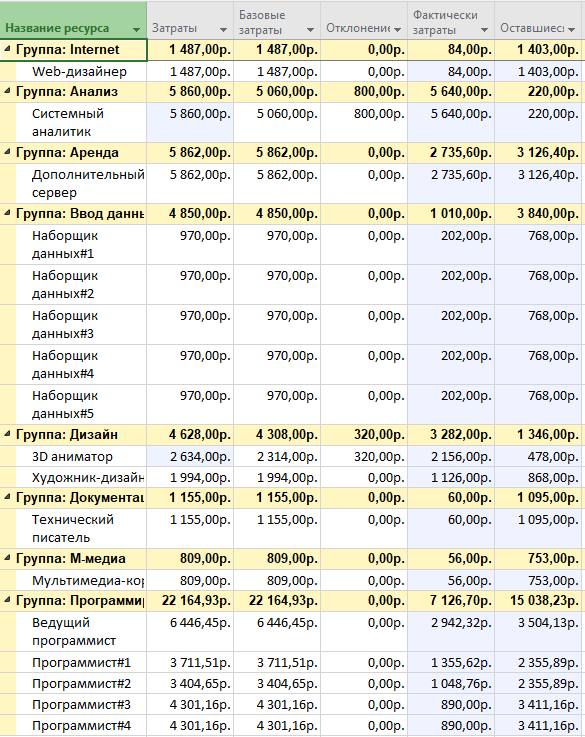
\includegraphics[width=0.7\linewidth]{src/4_4}
	\caption{}
	\label{fig:44}
\end{figure}

\section{Условия}
\begin{enumerate}
	\item Дата получения заданич 07.04
	\item Дата отчета 20 мая;
	\item Выставить выполненность задачи по текущей дате (кроме):
	\begin{enumerate}
		\item 30з - закончилось на 1 неделю позже;
		\item 33з - началась на 1 неделю позже;
		\item 35з - 20\% заверешно.
	\end{enumerate}
	\item Дополнительные условия:
	\begin{enumerate}
		\item Ведущий программист: с 1 апреля на 10 дней отправлен на повышении квалификации, работает на 20\%. После завершения зарплата вырастает на 10\%;
		\item С 20 апреля отказались от сервера и купили за 4000р;
		\item На совещании находятся текущие работники или те которые будут заняты в течении нескольких недель.
	\end{enumerate}
\end{enumerate}

\subsection{Задача 1}
Устанавливаем дату отчета на 20.05.2021г (см \ref{fig:411})
\begin{figure}[H]
	\centering
	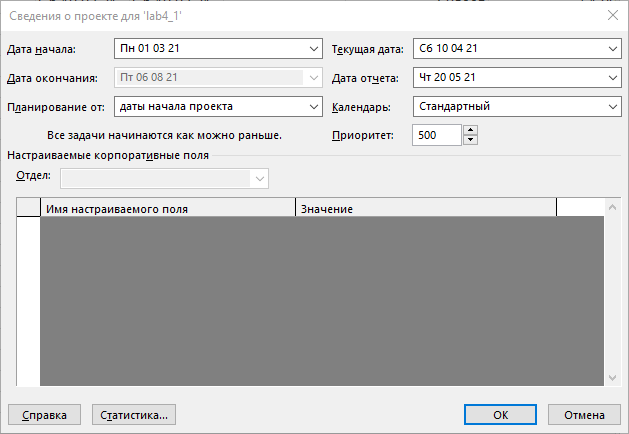
\includegraphics[width=0.7\linewidth]{src/4_1_1}
	\caption{Установка даты отчета}
	\label{fig:411}
\end{figure}


\subsection{Задача 2}
Обновляем проект (см \ref{fig:412}).
\begin{figure}[H]
	\centering
	
\includegraphics[width=0.7\linewidth]{src/4_1_2}
	\caption{Обновляем проект}
	\label{fig:412}
\end{figure}

Задача 30, закончилась на 1неделю позже.
Задача 33 началась позже на 1 неделю.
Зачада 35 на 20% завершено

Ведущий программист с 1 апреля на 10 дней отправлен на повышении квалификации, работает на 20\%. После завершения зарплата вырастает на 10\%;
Установим доступность "Ведущего программиста" с 1 - 10 апреля равной 20%;
\begin{figure}[H]
	\centering
	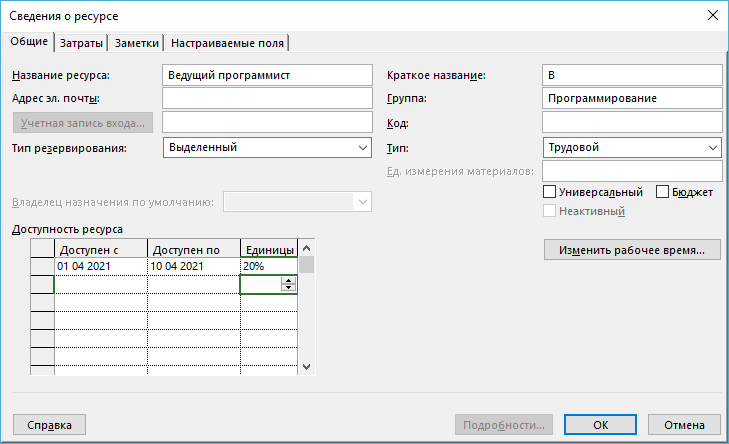
\includegraphics[width=0.7\linewidth]{src/4_5}
	\caption{Доступность ресурса}
	\label{fig:45}
\end{figure}


Начинаю с 11 числа его зарплата вырастает на 10\% (см \ref{fig:46} \ref{fig:47})
\begin{figure}[H]
	\centering
	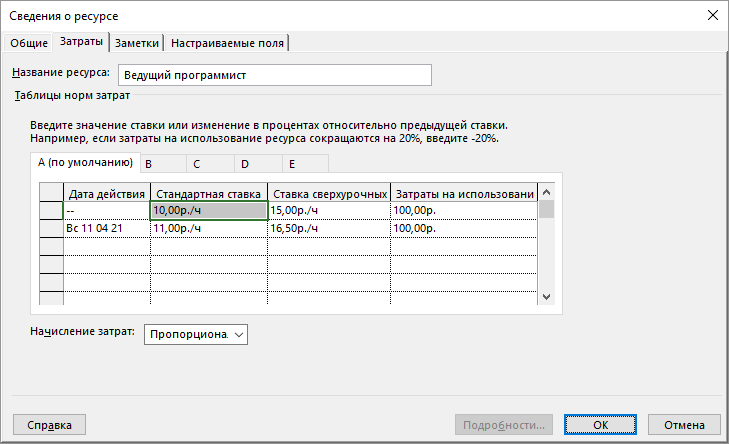
\includegraphics[width=0.7\linewidth]{src/4_6}
	\caption{Зарплата "Ведущего программиста"}
	\label{fig:46}
\end{figure}
\begin{figure}[H]
	\centering
	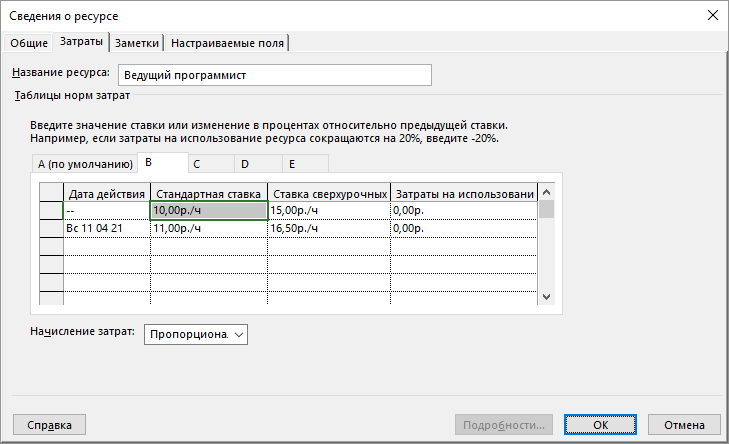
\includegraphics[width=0.7\linewidth]{src/4_7}
	\caption{Зарплата "Ведущего программиста"}
	\label{fig:47}
\end{figure}

В стоимость проекта возрасла на 1487рублей.
Время выполнения проекта не изменилось.

Начиная с 20 апреля отказались от аренды сервера и купили свой за 4000р.
Создадим новый ресурс под названием "Сервер" (\ref{fig:48}).
\begin{figure}[H]
	\centering
	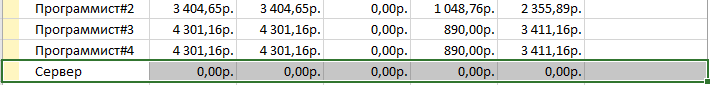
\includegraphics[width=0.7\linewidth]{src/4_8}
	\caption{Создадим ресурса "Сервер"}
	\label{fig:48}
\end{figure}

Считам что сервер был приобретен и установлен за 4000р и ровно 20 апреля был осуществлен переход на собственный.
В результате стоимость аренды сократилась на -4556р. Что дало нам съэкономить 554рубля.
Итоговая стоимость проекта возрасла на 939р.

Теперь обновомис список участников на совещаниях.
На совещаниях присутсвуют люди которые работаю или будут работать над заданиями (2 недели)

Список совещаний которые не будут посещаться сотрдуником:
\begin{enumerate}
	\item Ведущий программист: 09.06 - 07.07 (\ref{fig:410});
	\item Системный аналитек: 14.04 - окончание проекта;
	\item Художник дизайнер: 24.03 - 09.06, 07.07 - кп;
	\item Технический писатель: 03.03 - 16.06 и 4.08;
	\item Веб дизайнер: 03.03 - 16.06 и 4.08;
	\item 3D аниматор: 14.04 - 09.06, 07.07;
	\item Мультимедиа коресподент: 03.03 - 24.03, 02.06 - кп
\end{enumerate}

\begin{figure}[H]
	\centering
	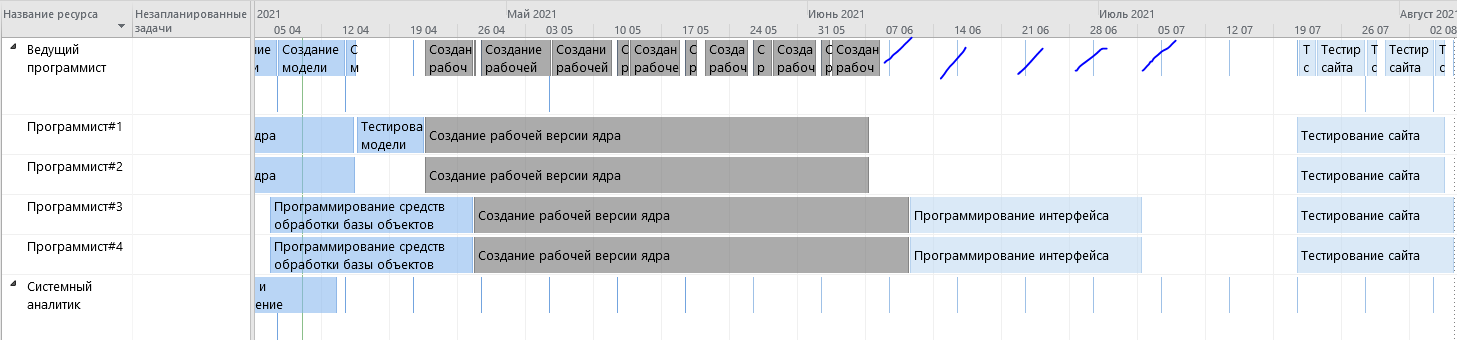
\includegraphics[width=0.7\linewidth]{src/4_10}
	\caption{Неактуальные совещания}
	\label{fig:410}
\end{figure}

В результате нам удалось съэкономить 491руб на совещании. 
В стоимость проекта возрасла на 431р.

\subsection{Задача 3}
\begin{figure}[H]
	\centering
	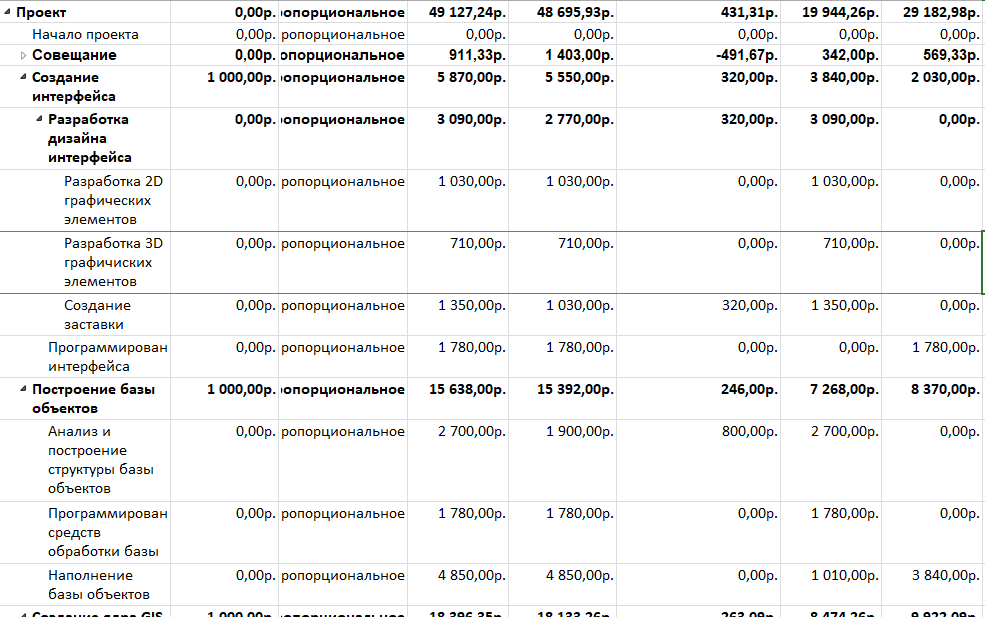
\includegraphics[width=0.7\linewidth]{src/4_11}
	\caption{}
	\label{fig:411}
\end{figure}
\begin{figure}[H]
	\centering
	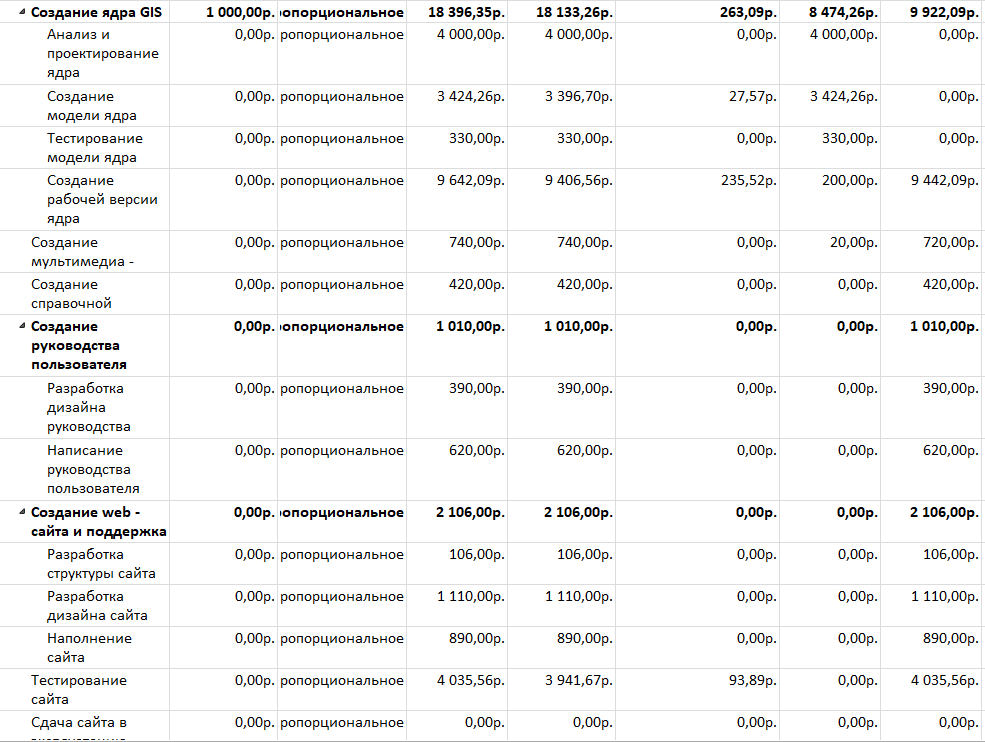
\includegraphics[width=0.7\linewidth]{src/4_12}
	\caption{}
	\label{fig:412}
\end{figure}

\subsection{Задача 4}
\begin{figure}[H]
	\centering
	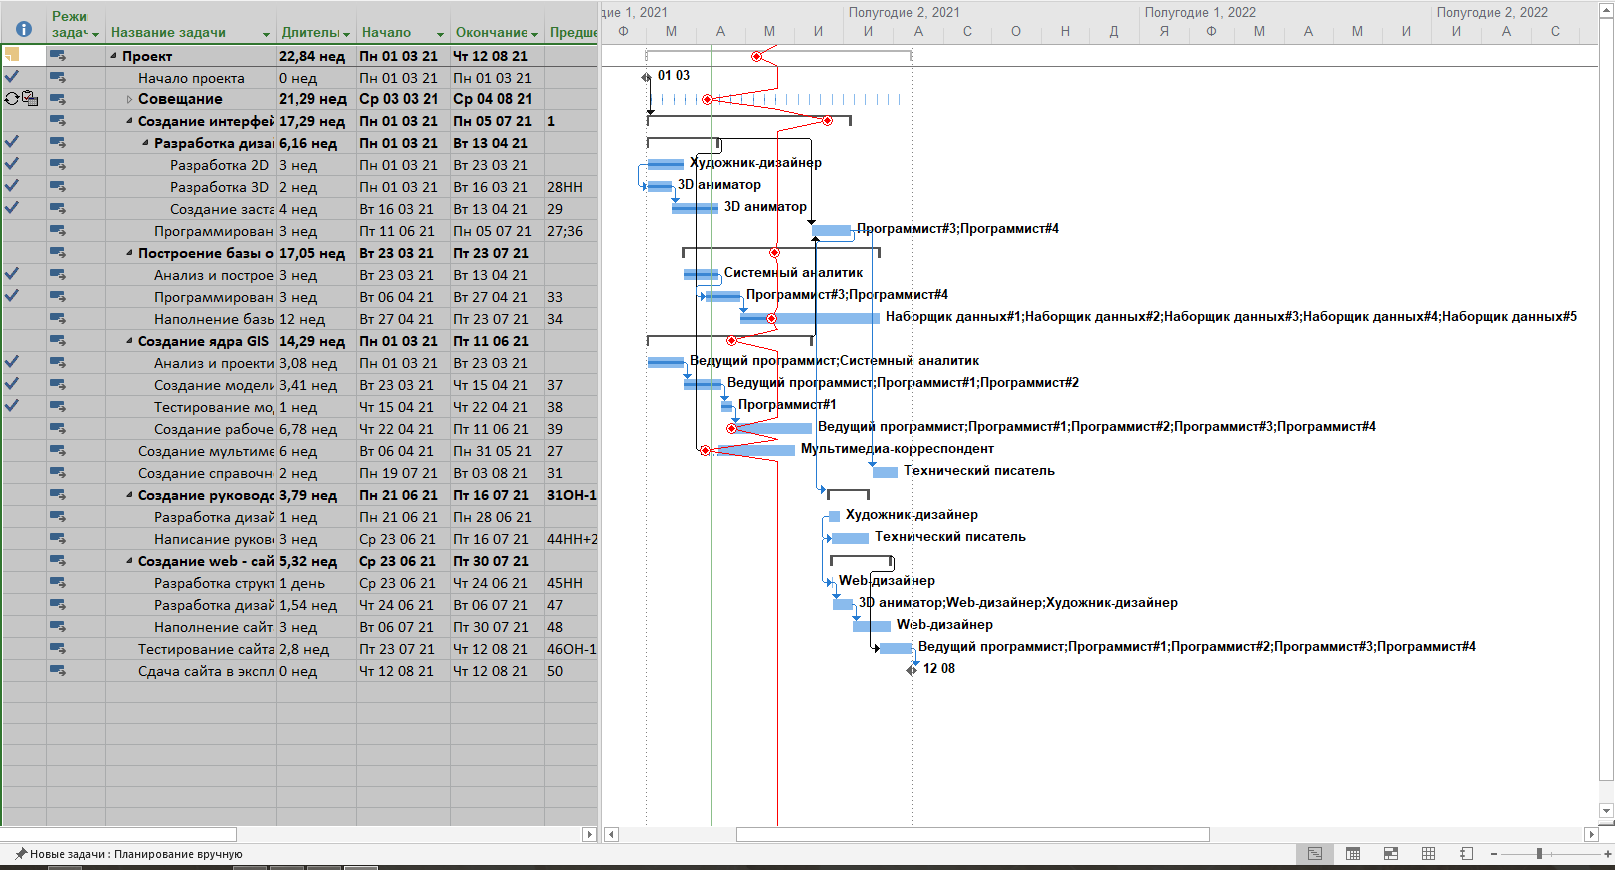
\includegraphics[width=0.7\linewidth]{src/4_13}
	\caption{Линия прогресса}
	\label{fig:413}
\end{figure}

\subsection{Задача 5}
Посмотрите, насколько проект отклонился от графика. 
Предложите стратегию устранения временных отклонений. 
Продемонстрируйте результаты ее применения на модели «Что-если». 
Результат сохраните в отдельном файле.








